% ==========================================
% BAB IV DESAIN KONSEP SOLUSI
% ==========================================
\chapter{DESAIN KONSEP SOLUSI}
\label{chap:desain-konsep-solusi}
Bab ini mengilustrasikan desain konsep solusi dalam bentuk model konseptual dan penjelasan secara ringkas, beserta perbedaannya dengan sistem saat ini. Bab ini berisi gambar desain konsep solusi tersebut dan penjelasan perbandingannya dengan gambar sistem yang ada saat ini (yang tergambar di awal Bab \ref{chap:analisis-masalah}).

\section{Analisis Kondisi Audit Energi yang Akan Datang}
Kondisi yang akan datang dirancang berdasarkan solusi terpilih pada Bab sebelumnya, yaitu pengembangan perangkat lunak audit energi berbasis aplikasi web luring dengan sinkronisasi otomatis. Pemilihan solusi ini dapat menjawab permasalahan utama pada proses audit energi, seperti ketergantungan pada pencatatan manual, ketidakteraturan format data, keterbatasan validasi, serta tidak tersedianya penyimpanan histori audit yang terpusat. Pendekatan ini memungkinkan aplikasi berjalan melalui peramban web namun tetap memiliki kemampuan penyimpanan lokal dan sinkronisasi data, sehingga sesuai dengan kondisi audit lapangan yang sering dilakukan pada lokasi dengan keterbatasan konektivitas jaringan.

Dengan pendekatan aplikasi web luring, proses pengumpulan dan pengolahan awal data audit tidak lagi bergantung pada koneksi internet secara terus-menerus. Data dapat diinput, divalidasi, dan disimpan secara lokal di perangkat pengguna, kemudian disinkronkan ke server pusat ketika koneksi tersedia. Perubahan alur kerja ini meningkatkan efisiensi proses audit, mengurangi risiko kehilangan data, serta memastikan bahwa perhitungan indikator dan penilaian dilakukan secara terstandar oleh sistem. Ilustrasi alur proses audit energi yang diusulkan ditunjukkan pada Gambar~\ref{gambar:proses-audit-yang-akan-datang}, yang merepresentasikan kondisi proses audit energi setelah penerapan solusi perangkat lunak yang diusulkan.

\begin{figure}[H]
    \centering
    \captionsetup{justification=centering}
        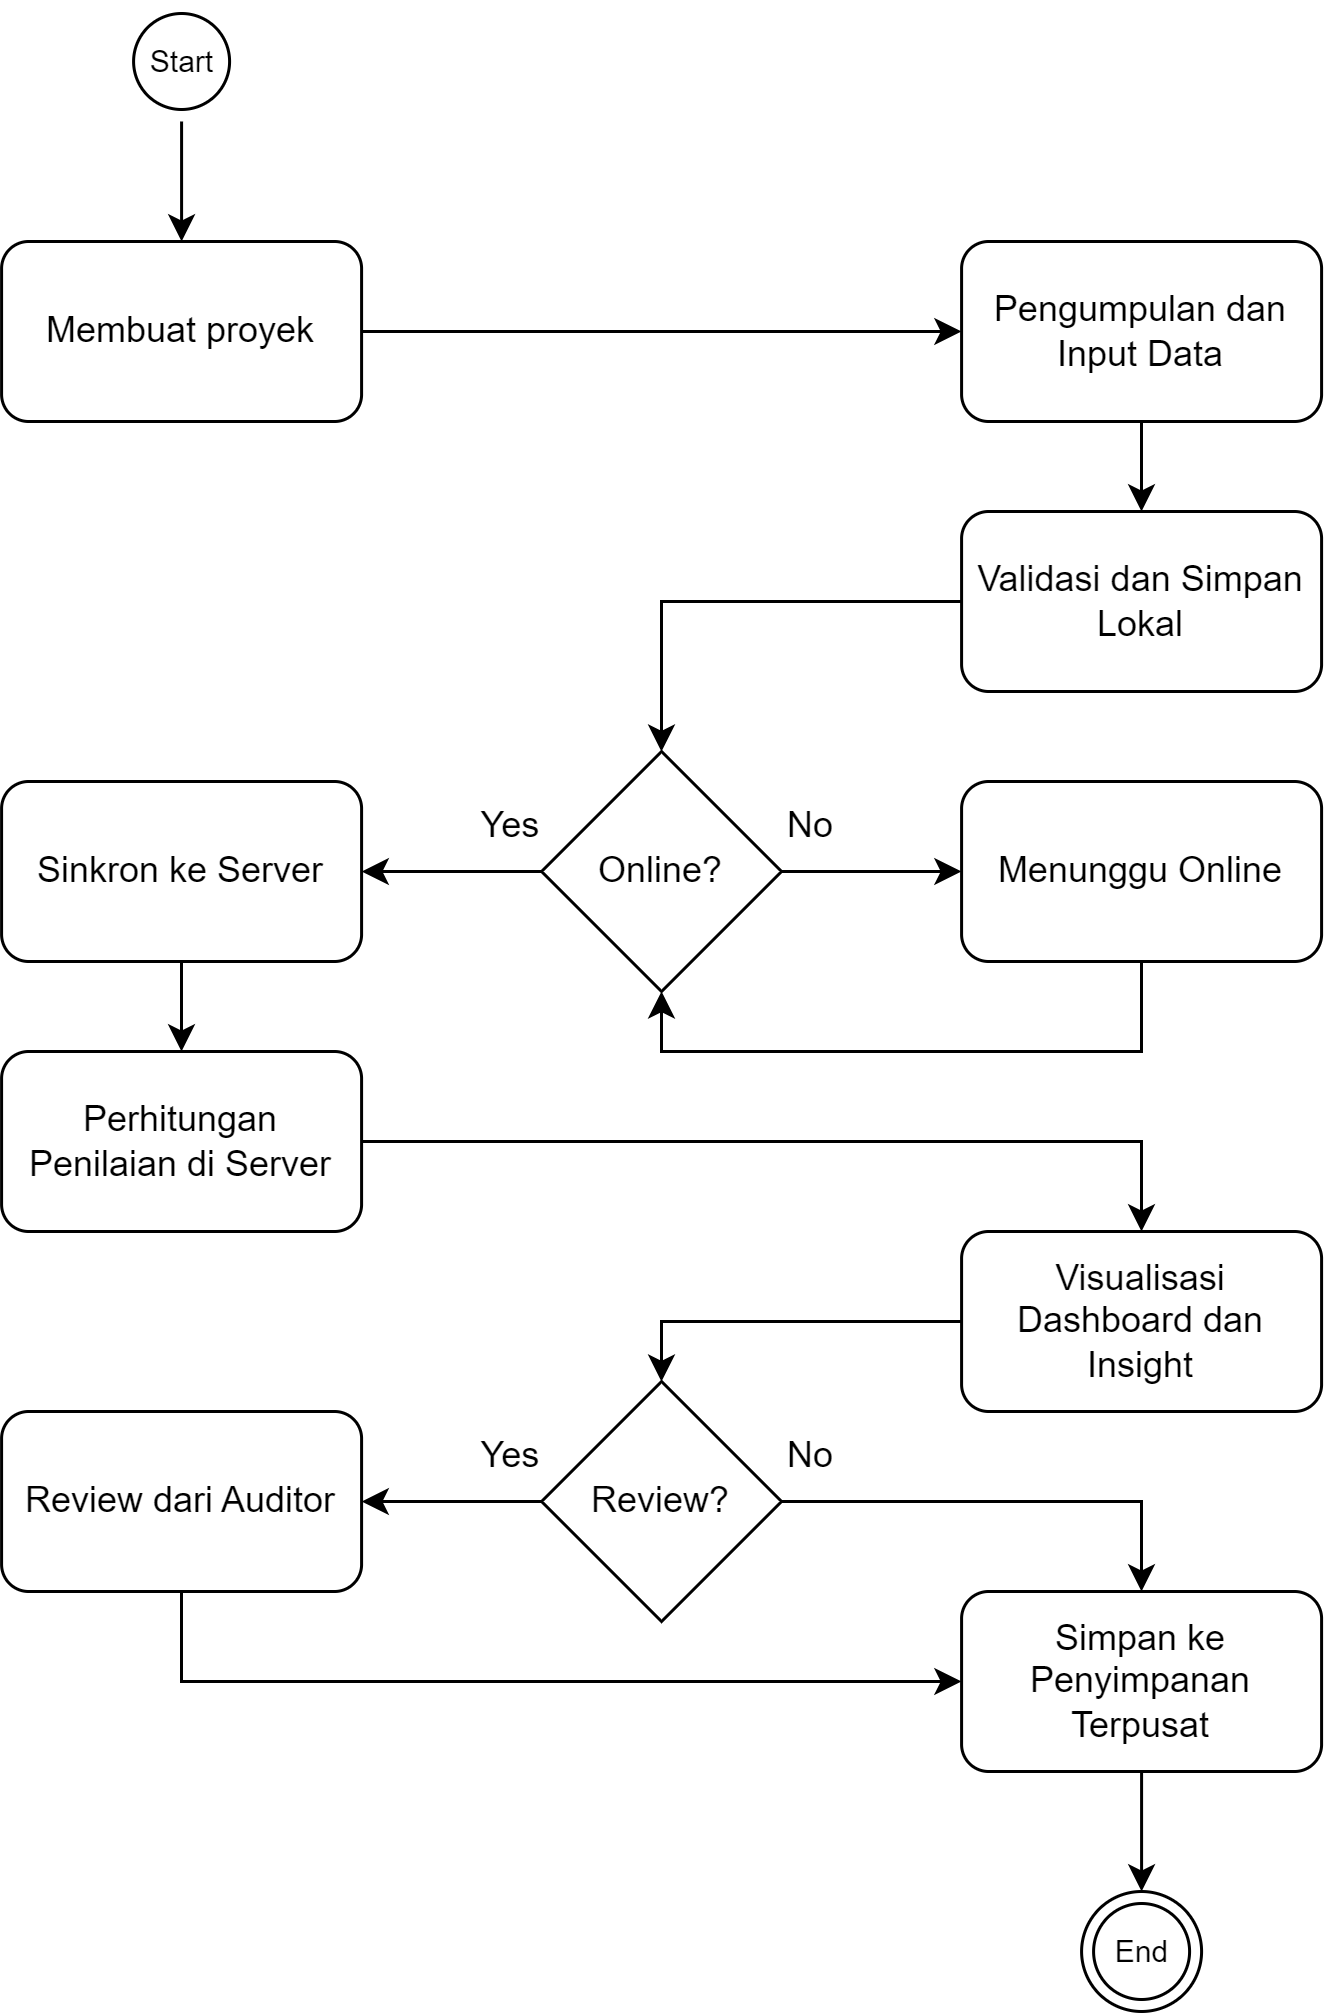
\includegraphics[width=0.7\textwidth]{image/to-be}
    \caption{Diagram Aktivitas Proses Audit Energi yang Akan Datang}
    \label{gambar:proses-audit-yang-akan-datang}
\end{figure}

Berdasarkan Gambar~\ref{gambar:proses-audit-yang-akan-datang}, proses audit energi pada kondisi yang akan datang diawali dengan membuat proyek audit, yang berfungsi sebagai wadah untuk mendefinisikan ruang lingkup, periode audit, serta identitas bangunan yang diaudit. Tahap ini menggantikan pencatatan terpisah pada sistem manual dan menjadi dasar pengelolaan data audit secara terstruktur. Selanjutnya, pengumpulan dan input data audit dilakukan melalui perangkat lunak secara luring, sehingga auditor dapat melakukan pencatatan data lapangan tanpa bergantung pada ketersediaan jaringan.

Data yang diinput akan melalui proses validasi dan disimpan secara lokal di perangkat pengguna. Mekanisme ini memastikan bahwa data telah memenuhi aturan dasar sebelum dikirimkan ke sistem terpusat, serta mengurangi potensi kesalahan input yang umum terjadi pada proses berbasis \textit{spreadsheet}. Proses sinkronisasi data dilakukan ketika koneksi tersedia, di mana seluruh data lokal yang telah tervalidasi dikirim ke server pusat. Pendekatan ini memungkinkan integrasi data secara bertahap tanpa mengganggu aktivitas audit lapangan.

Pada sisi server, sistem menjalankan perhitungan indikator kinerja energi dan mekanisme penilaian secara otomatis dan terstandar. Pemusatan proses perhitungan ini memastikan konsistensi metode analisis antar audit dan antar periode waktu. Hasil perhitungan disajikan dalam bentuk \textit{dashboard} dan laporan otomatis yang dapat diakses oleh auditor dan pengelola gedung untuk mendukung proses evaluasi dan pengambilan keputusan. Seluruh hasil audit kemudian disimpan dalam basis data terpusat sebagai histori audit, sehingga memungkinkan evaluasi berkala, perbandingan antar periode, serta analisis tren konsumsi energi secara berkelanjutan.

\section{Perbandingan Kondisi Audit Energi Saat Ini dan Kondisi yang Akan Datang}
Perbandingan antara kondisi proses audit energi saat ini dan kondisi yang akan datang disajikan pada Tabel~\ref{tbl:perbandinganasisdantobe} untuk menegaskan perubahan mendasar yang diusulkan melalui pengembangan perangkat lunak audit energi yang difokuskan pada aspek-aspek operasional.

\input table/tabelperbandinganasisdantobe.tex

Berdasarkan Tabel~\ref{tbl:perbandinganasisdantobe}, kondisi yang akan datang menunjukkan pergeseran signifikan dari proses audit energi yang bersifat manual menuju sistem yang lebih terstruktur dan terintegrasi. Pengumpulan dan penginputan data yang sebelumnya bergantung pada pencatatan manual dan \textit{spreadsheet} digantikan dengan mekanisme input terstandar yang mendukung operasi luring, sehingga meningkatkan konsistensi data dan mengurangi hambatan akibat keterbatasan konektivitas. Proses validasi awal dan perhitungan indikator dilakukan secara otomatis oleh sistem, yang membantu menekan potensi kesalahan perhitungan serta mempercepat tahapan analisis. Penyajian hasil audit dalam bentuk \textit{dashboard} dan laporan otomatis, serta penyimpanan histori audit secara terpusat, memberikan dukungan yang lebih baik untuk evaluasi berkala dan pengambilan keputusan berbasis data pada pengelolaan energi gedung.

\section{Desain Fungsional Sistem Perangkat Lunak Audit Energi}
Desain fungsional sistem disusun untuk menggambarkan bagaimana perangkat lunak penilaian yang diusulkan mendukung proses audit energi melalui fungsi-fungsi utama yang terstruktur. Pada tahap ini dilakukan identifikasi aktor yang terlibat serta perancangan interaksi antara aktor dan sistem dalam menjalankan proses audit energi. Pendefinisian aktor diperlukan untuk memperjelas peran, batasan akses, dan tanggung jawab masing-masing pihak, sehingga desain fungsional yang dihasilkan mencerminkan kebutuhan penggunaan sistem secara nyata. Definisi aktor yang terlibat dalam sistem audit energi disajikan pada Tabel~\ref{tbl:actor}.

\input table/tabelaktor.tex

Berdasarkan definisi aktor pada Tabel~\ref{tbl:actor}, sistem audit energi melibatkan dua peran utama dengan tingkat interaksi yang berbeda, yaitu auditor energi dan pengelola gedung. Auditor energi berperan sebagai pengguna utama yang menginisiasi dan mengendalikan proses audit melalui pengelolaan proyek dan penginputan data audit. Pengelola gedung berperan sebagai pengguna yang memanfaatkan keluaran sistem, khususnya untuk memantau hasil audit dalam bentuk \textit{dashboard} dan laporan sebagai dasar pengambilan keputusan operasional. Perbedaan peran dan akses ini diilustrasikan melalui diagram \textit{use case} yang ditampilkan pada Gambar~\ref{gambar:usecase}, yang menggambarkan cakupan fungsi sistem serta hubungan antara aktor dan fungsi-fungsi utama yang disediakan oleh perangkat lunak audit energi.

\begin{figure}[H]
    \centering
    \captionsetup{justification=centering}
        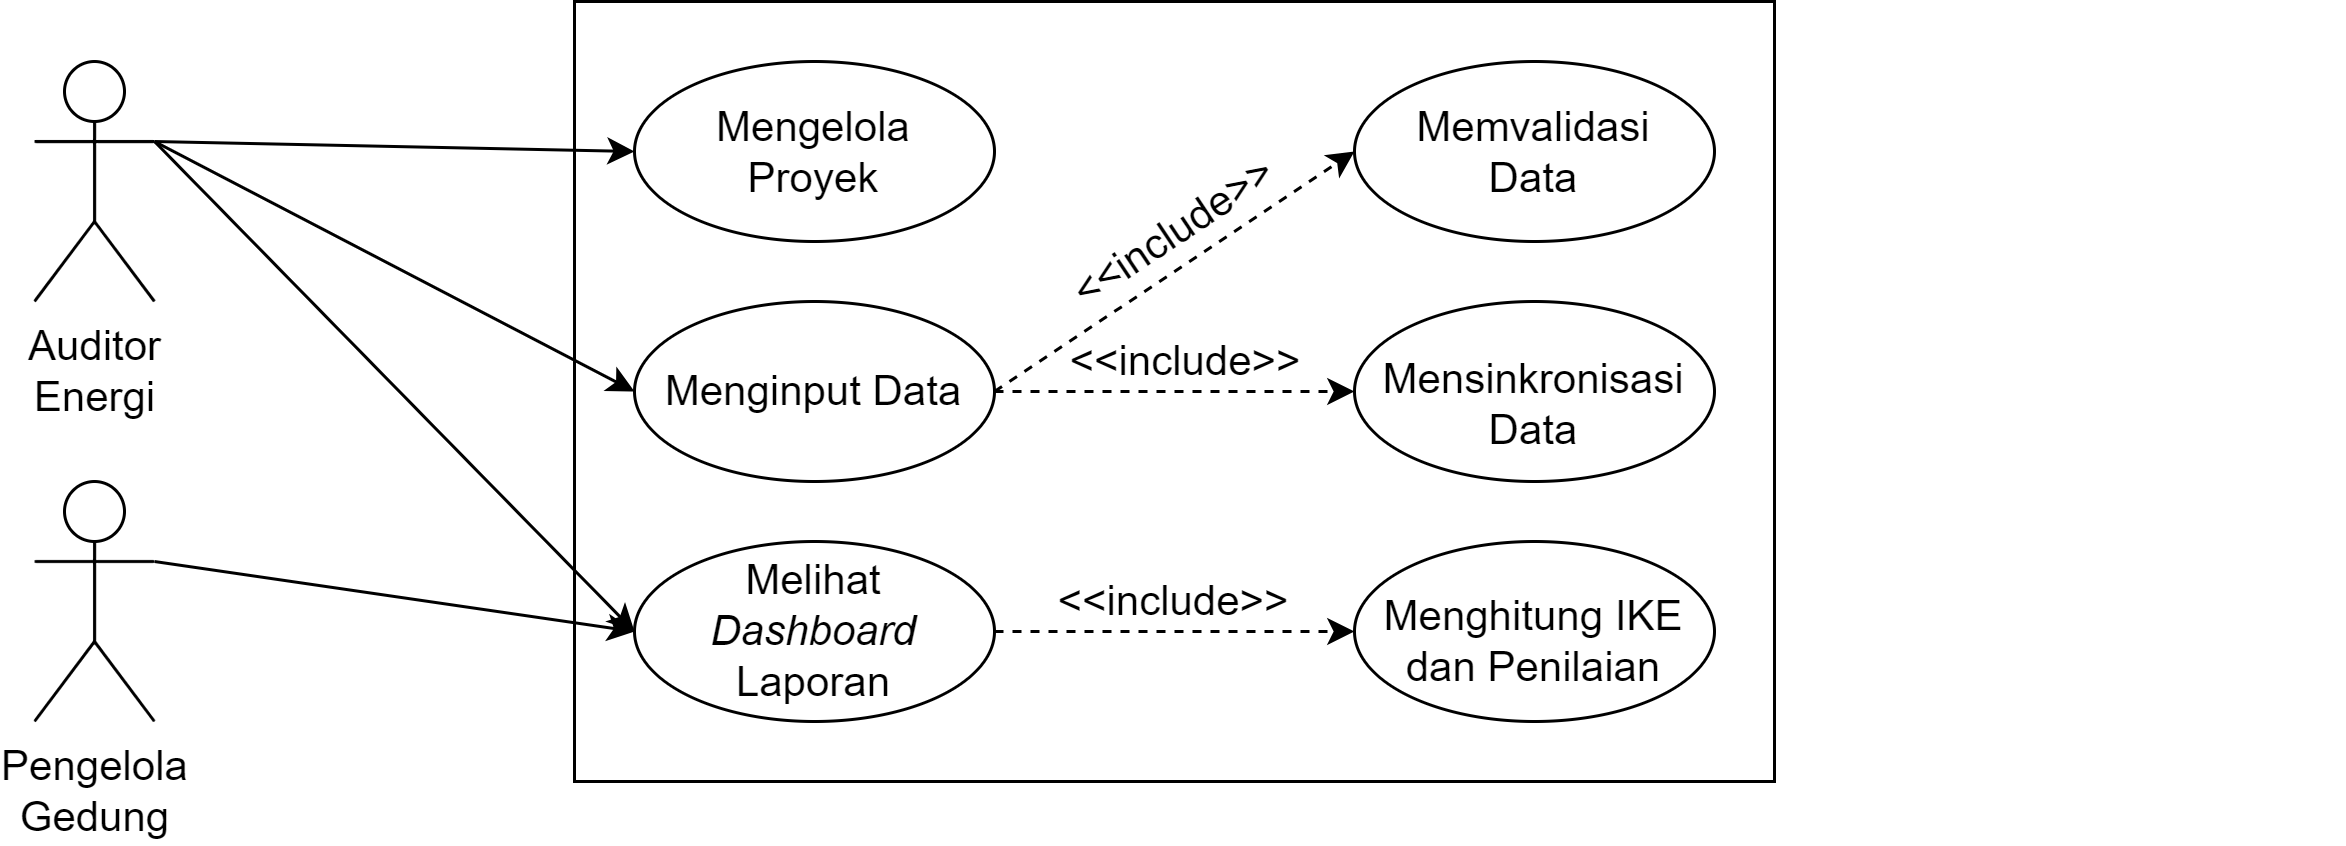
\includegraphics[width=0.95\textwidth]{image/usecase}
    \caption{Diagram \textit{Use Case} Perangkat Lunak Audit Energi}
    \label{gambar:usecase}
\end{figure}

Diagram \textit{use case} pada Gambar~\ref{gambar:usecase} menampilkan fungsi-fungsi utama yang disediakan oleh sistem audit energi beserta hubungan interaksinya dengan masing-masing aktor. Auditor energi berinteraksi dengan sistem untuk mengelola proyek audit, melakukan penginputan data, serta mengakses hasil audit. Beberapa proses teknis, seperti validasi data, sinkronisasi data, serta perhitungan indikator kinerja energi dan penilaian, dimodelkan sebagai \textit{use case} yang di-\textit{include} dan dijalankan secara otomatis oleh sistem sebagai bagian dari alur internal, sehingga tidak memerlukan interaksi langsung dari aktor. Pengelola gedung hanya terhubung dengan fungsi pemantauan hasil audit melalui \textit{dashboard} dan laporan, sesuai dengan perannya sebagai pengguna keluaran sistem. Definisi dari setiap \textit{use case} yang ditampilkan dalam diagram \textit{use case}, termasuk deskripsi dan keterkaitannya dengan kebutuhan fungsional sistem dan juga aktornya dijelaskan lebih lanjut pada Tabel~\ref{tbl:uc}.

\input table/tabeluc.tex

Berdasarkan definisi \textit{use case} pada Tabel~\ref{tbl:uc}, dapat dilihat bahwa desain fungsional sistem audit energi ini diturunkan secara langsung dari kebutuhan fungsional yang telah dirumuskan pada tahap analisis kebutuhan. Setiap \textit{use case} merepresentasikan fungsi inti yang diperlukan untuk mendukung proses audit energi secara terstruktur, mulai dari pengelolaan proyek dan data audit hingga penyajian hasil dalam bentuk \textit{dashboard} dan laporan. Desain ini menegaskan peran sistem sebagai pendukung audit yang mengotomasi proses teknis dan perhitungan, sementara auditor tetap berperan dalam interpretasi hasil dan pengambilan keputusan. Dengan demikian, desain fungsional sistem ini menjadi dasar yang jelas dan terdefinisi untuk tahap perancangan detail dan implementasi perangkat lunak pada tahap selanjutnya.

\section{Desain Data Sistem Perangkat Lunak Audit Energi}
Desain data sistem disusun untuk menggambarkan struktur data yang digunakan dalam perangkat lunak audit energi, termasuk entitas utama, atributnya, serta hubungan antar entitas. Desain ini penting untuk memastikan bahwa data yang dikumpulkan, diproses, dan disimpan oleh sistem dapat dikelola secara efisien dan mendukung kebutuhan fungsional yang telah ditetapkan. Pada tahap ini dilakukan identifikasi entitas utama yang relevan dengan proses audit energi, seperti proyek audit, data audit, hasil perhitungan indikator, serta histori audit. Hubungan antar entitas juga dirancang untuk mencerminkan alur data yang terjadi selama proses audit, mulai dari input data hingga penyimpanan hasil audit. Hubungan antar entitas ini diilustrasikan melalui diagram entitas-relasi yang ditampilkan pada Gambar~\ref{gambar:er}.

\begin{figure}[H]
    \centering
    \captionsetup{justification=centering}
        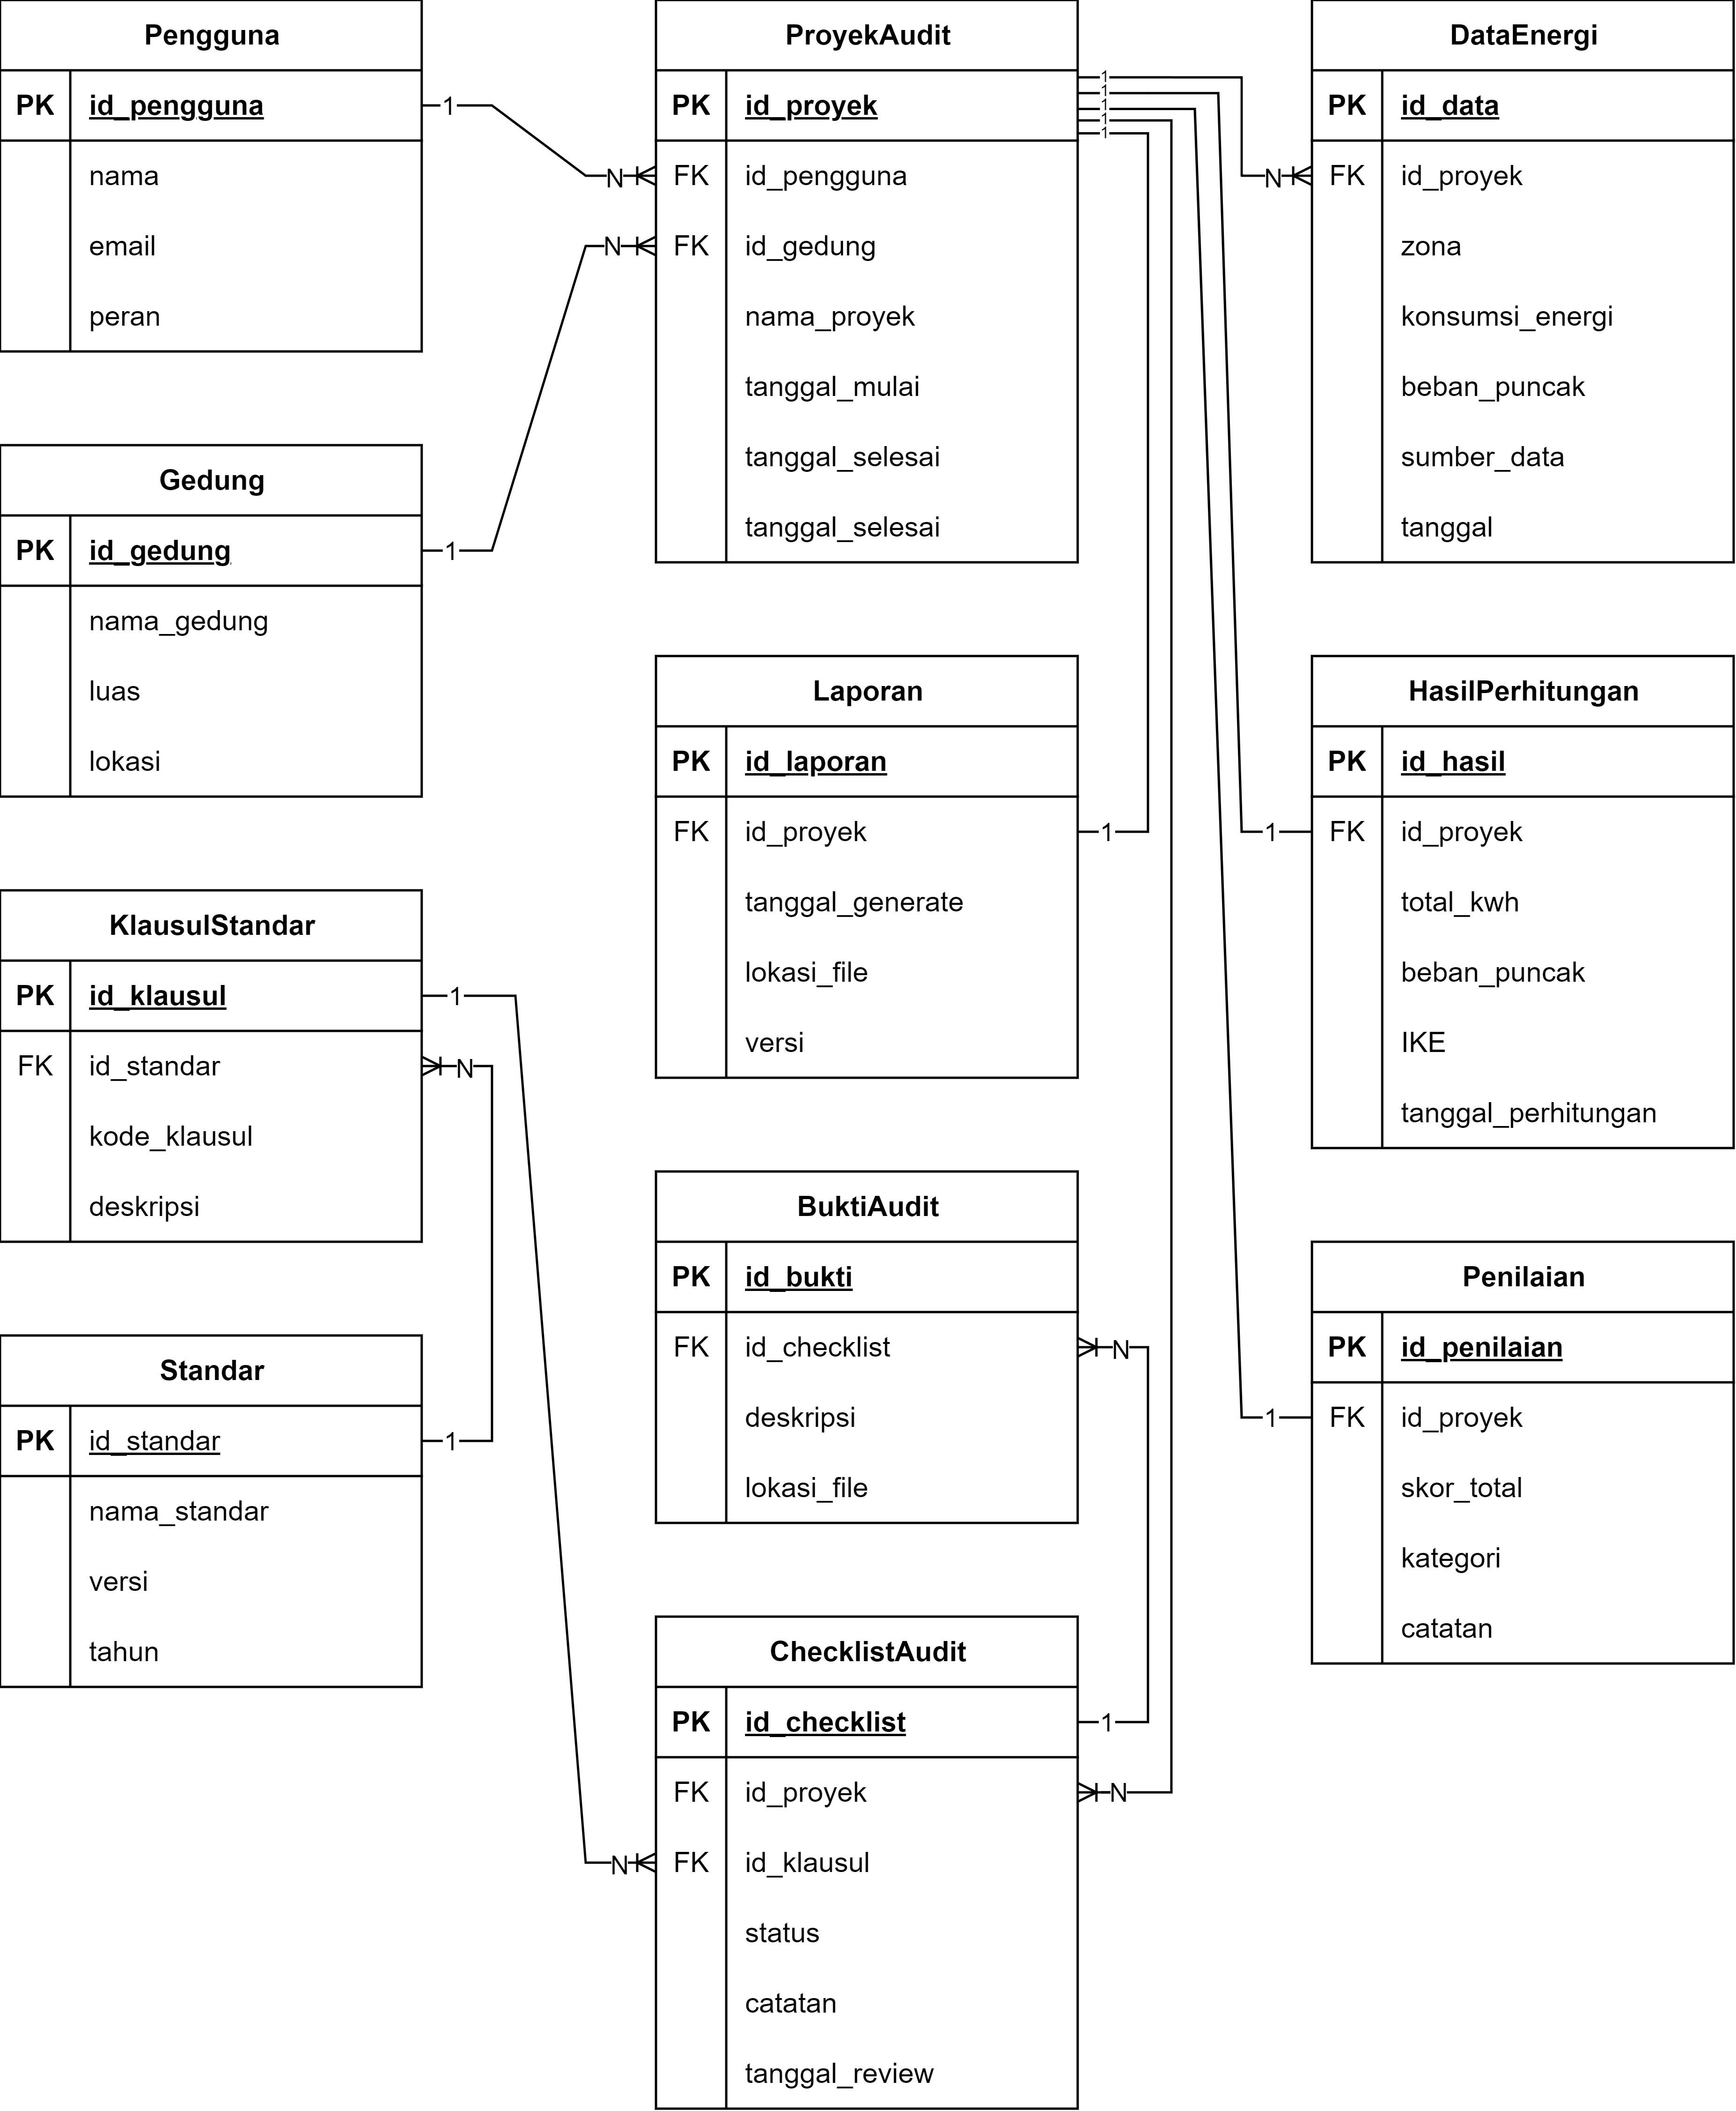
\includegraphics[width=0.95\textwidth]{image/er}
    \caption{Diagram Entitas-Relasi Perangkat Lunak Audit Energi}
    \label{gambar:er}
\end{figure}

Diagram entitas-relasi pada Gambar~\ref{gambar:er} menampilkan struktur data utama yang digunakan dalam sistem audit energi serta hubungan antarentitas yang terlibat dalam proses pengelolaan data audit. Melalui diagram tersebut dapat dilihat bahwa sistem menyimpan informasi mengenai pengguna, proyek audit, objek gedung yang diaudit, data energi yang dikumpulkan selama proses audit, serta hasil perhitungan indikator dan penilaian yang dihasilkan oleh sistem. Selain itu, model data juga mencakup entitas yang berkaitan dengan kepatuhan terhadap standar audit energi, seperti standar, klausul standar, checklist audit, dan bukti audit, yang mendukung proses dokumentasi audit secara lebih terstruktur. Definisi dari setiap entitas yang terdapat dalam diagram pada Gambar~\ref{gambar:er} dijelaskan lebih lanjut pada Tabel~\ref{tbl:entitas}.

\input table/tabelentitas.tex

Berdasarkan definisi entitas pada Tabel~\ref{tbl:entitas}, model data sistem audit energi dirancang untuk mendukung seluruh proses utama yang telah diidentifikasi pada tahap analisis kebutuhan, mulai dari pengelolaan proyek audit, pengumpulan data energi, perhitungan indikator kinerja energi, hingga penyusunan laporan audit. Struktur relasi antarentitas memungkinkan sistem menyimpan data audit secara terorganisasi serta mendukung penelusuran histori audit pada periode yang berbeda. Dengan demikian, desain data ini menjadi dasar bagi implementasi basis data sistem audit energi sekaligus memastikan bahwa kebutuhan fungsional yang telah dirumuskan pada tahap sebelumnya dapat diakomodasi secara konsisten dalam pengelolaan data sistem.